\documentclass{jsme-tj}

\usepackage{bm}
\newcommand{\Frac}[2]{\frac{\displaystyle #1}{\displaystyle #2}}

\title{Improved contact tracking algorithm for the omni wheel in general case 
of roller orientation}


\vol{1}
\no{1}
\field{XXX}

\received{0000/00/00}{XX-XXXX}


\author{x}{Ivan KOSENKO}
\author{y}{Sergey STEPANOV}
\author{z}{Kirill GERASIMOV}

\affiliate{x}{Department of Theoretical Mechanics, Moscow Aviation Institute 
(National Research University)}{Volokolamskoe shosse 4, Moscow, 125993, Russia}
[kosenko@ccas.ru]%
\affiliate{y}{Department of Mechanics, Institution of Russian Academy of 
Sciences Dorodnicyn Computing Centre of RAS}{Vavilov street 40, Moscow, 119333, 
Russia}
\affiliate{z}{Department of Theoretical Mechanics and Mechatronics, Lomonosov 
Moscow State University}{GSP-1, 1-52, Leninskie Gory, Moscow, 119991, Russia}

\begin{document}

\maketitle

\begin{abstract}
A multibody dynamics model for an omni wheel keeping its vertical orientation 
permanently in time is under development and verification. Such vertical 
positioning of the wheel plane is guaranteed if for instance the wheel belongs
to the larger multibody system, wheeled vehicle, rolling on the horizontal
floor. Contact tracking algorithms consume essential CPU time while simulating
dynamics of the multibody system. So development of new efficient algorithms of
this type is of actual interest. For instance it becomes possible in case of 
the omni vehicle moving on the horisontal surface. In this case contact 
tracking algorithm is possible to become specially ``simple'' and efficient. 
Base classes developed earlier for the multibody applications with contacts 
involving friction are used. A generalization has been performed for the former 
model of contact tracking algorithm between roller and horizontal floor. This 
generalization includes non-zero angle between the roller axis of rotation and 
plane of the omni wheel. Contact tracking algorithm is implemented in two 
cases: (a) implicit and (b) explicit. Computer models for these cases (a) and 
(b) are currently ``embedded'' into the omni wheel model earlier verified. Thus 
for simplicity we analyze a multibody system comprising the wheel plus set of 
rollers being mounted along its circumference. A remainder of the vehicle is 
replaced by the wrench properly arranged in a way such that the wheel keeps its 
vertical orientation permanently in time. The experimental computations 
performed have shown that two algorithms of the contact tracking generate 
completely identical dynamics of the whole multibody system.
\end{abstract}

\begin{keywords}
Omni wheel, Contact tracking, Unilateral constraint, Angled rollers, Model of 
friction.
\end{keywords}

\section{Introduction}

A construct of the omni vehicle~(Ilon, 1975) dynamical model has been presented 
in~(Kosenko, 2015), see also for instance papers~(K\'alm\'an, 2013), 
(Komori~et~al, 2016), (Tobolar, 2009), (Zobova and Tatarinov, 2009). Simplified 
model for the roller mounting on the wheel disk has been implemented there: the 
roller axis of rotation assumed to be in the disk, or equivalently the angle 
between this axis and the wheel plane, denote it by $\psi $, is equal to zero. 
We will call this angular parameter of the model as the angle of the 
preliminary roller rotation (pre-rotation). This pre-rotation supposed about 
the wheel radius intersecting the roller axis of rotation at its central point.

Omni wheel for this case is shown in Fig.~\ref{figure1}. There one can 
see the lateral view, fragment~(a), of the wheel being equipped by four 
axisymmetrical rollers. These rollers have been enumerated by their numbers. 
Each roller is connected to the wheel by a joint which axis coincides with the 
roller axis of rotation. This latter axis is orthogonal to the wheel radius 
exiting from the wheel central point $O$ and passing through the the roller 
central point. So it is possible for the wheel to have a free rolling in 
direction lateral to its plane. Corresponding contacting curve with respect to 
(w.~r.~t.) the wheel coordinate system, being a circle in the case shown, has a 
coloured highlighting. This curve has a circular shape provided the wheel plane 
keeps its vertical orientation. Front view of the omni wheel is shown in 
fragment~(b).

\begin{figure}[t]
\begin{center}
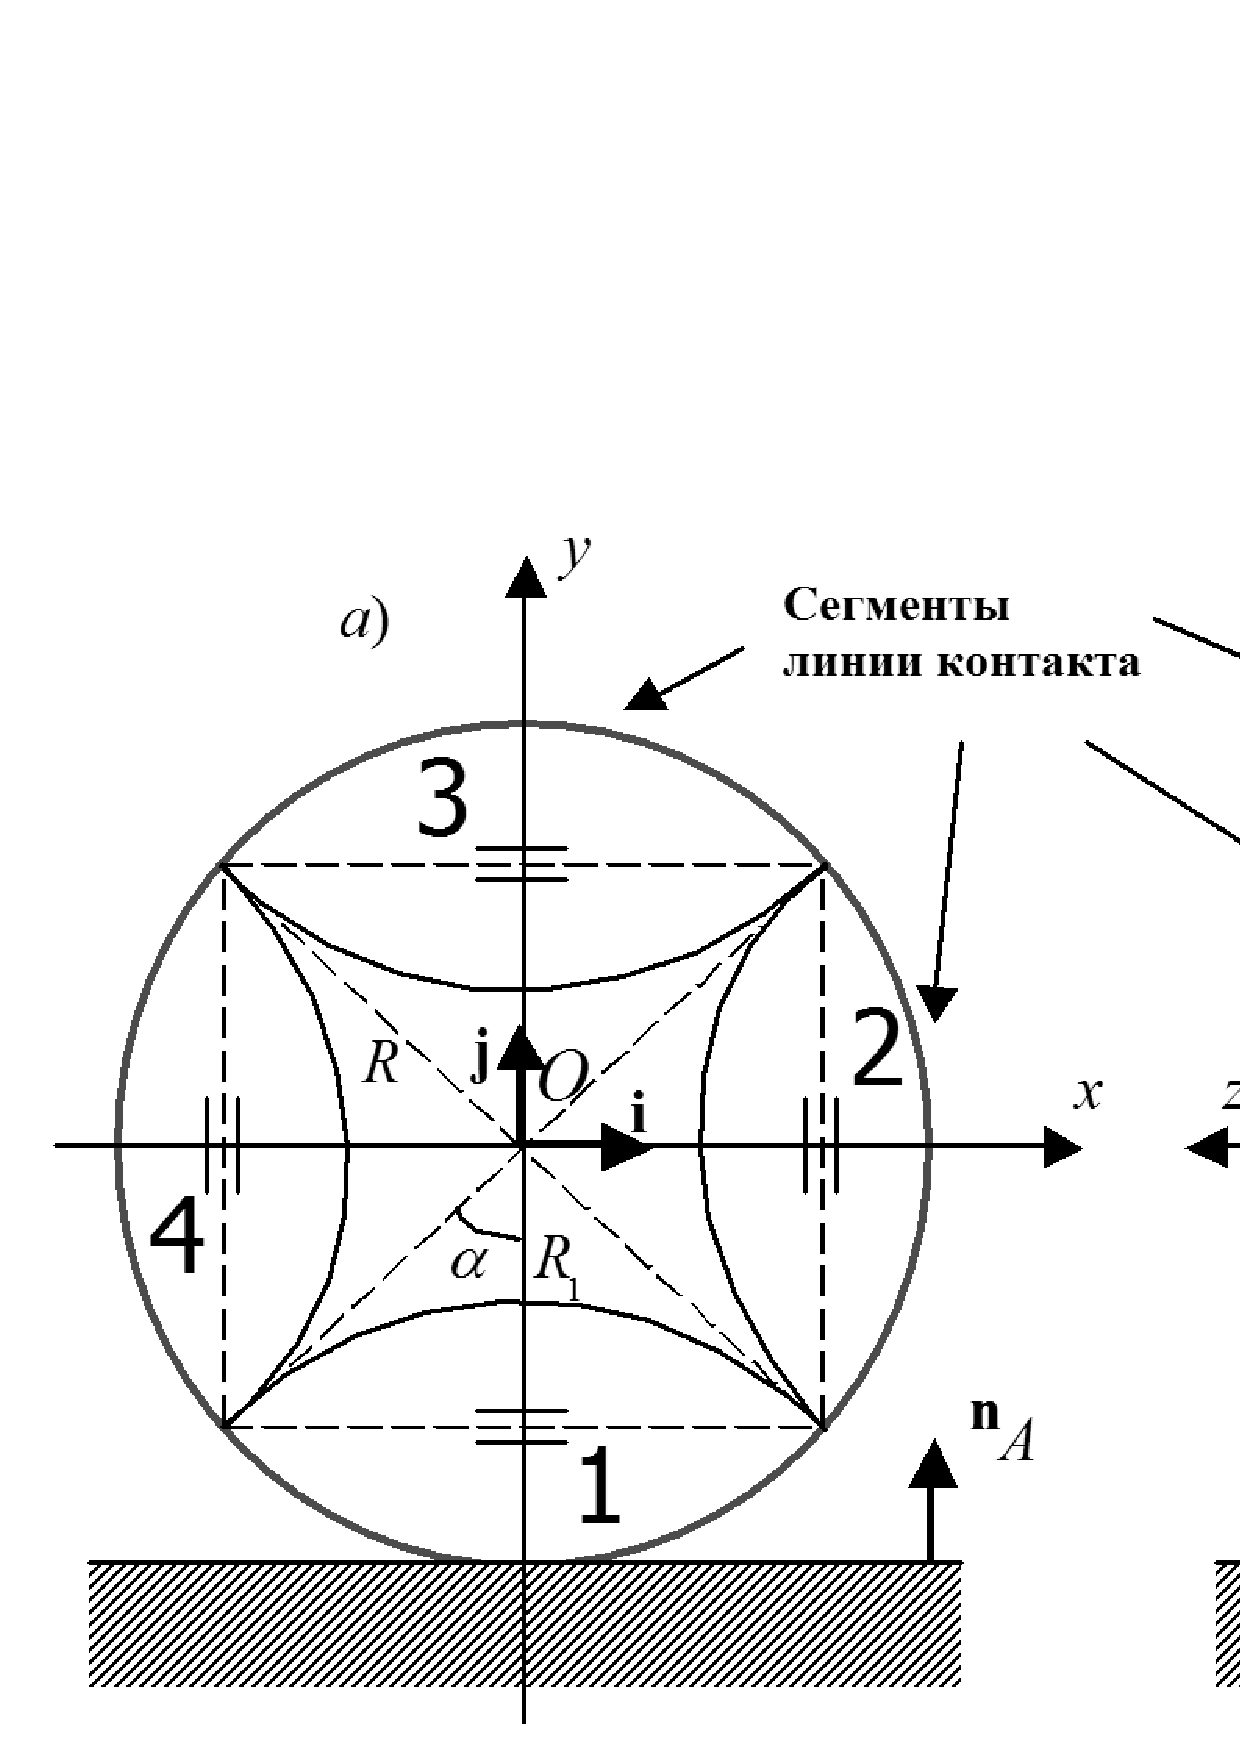
\includegraphics[bb= 0 0 19.50cm 16cm,scale=0.55]{OmniWheel.png}
%\centerline{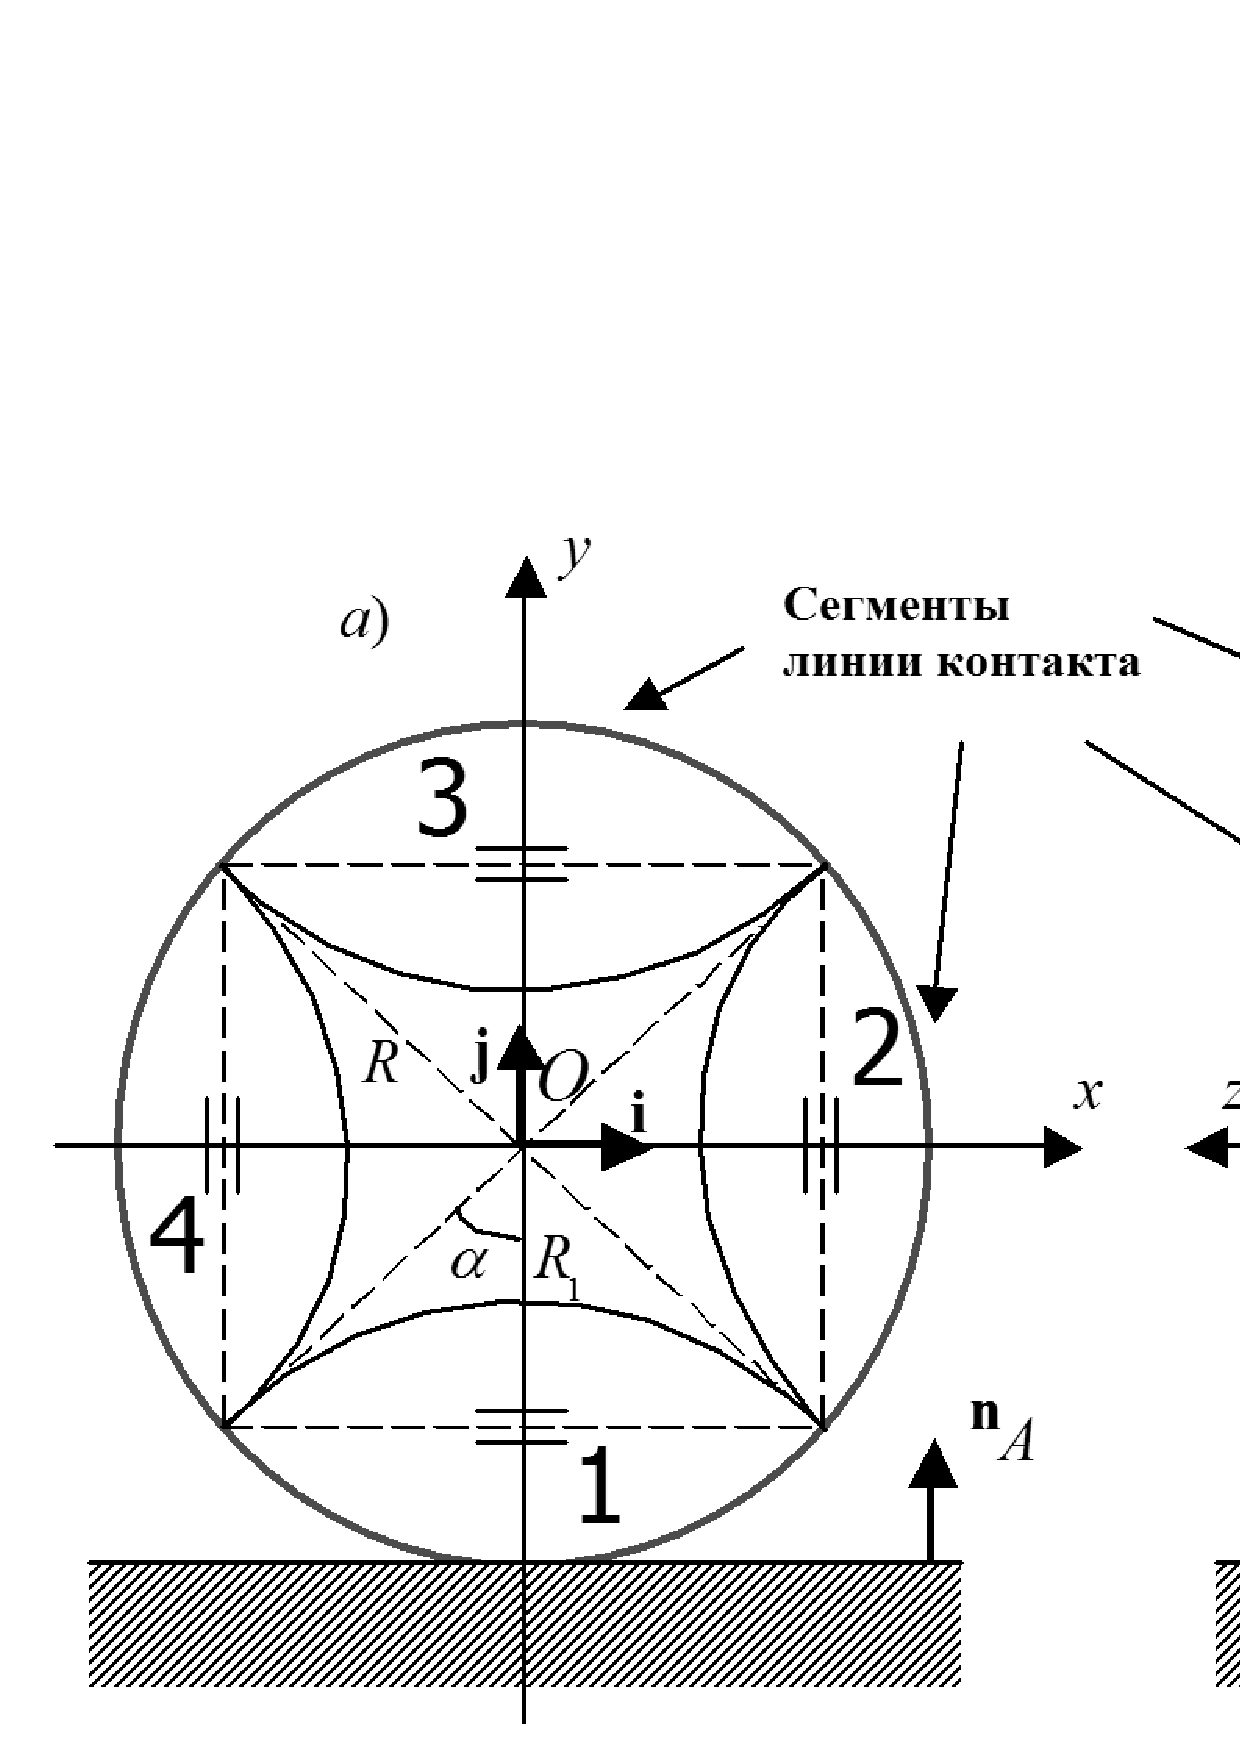
\includegraphics[bb= 0 0 19.50cm 16cm,scale=0.55]{OmniWheel.png}}
\caption{The omni wheel vertically aligned: (a) lateral view; (b) front view.}
\end{center}
\label{figure1}
\end{figure}

For the case of $\psi =0$ being shown in Fig.~\ref{figure1} a roller outer 
profile, generatrix, along its axis of rotation has evidently a circular shape, 
see Fig.~\ref{figure1}, fragment (a), again. This shape provides smooth 
transfer from one roller to another when moving. Evidently if $\psi\ne 0$ then 
the generatrix is not the circular segment. Thus, the contact tracking 
algorithm for the case of $\psi =0$ implemented in~(Kosenko, 2015) turned out 
to be simple enough. In the case of $\psi >0$ it becomes visibly complicated. 
And its implementation on Modelica language is the main goal of this paper.

Other details of Fig.~\ref{figure1} are the following: $R$ is the omni 
wheel radius, $R_1$ is the distance between the wheel central point $O$ and the 
roller central point, $\alpha $ is the half roller angular length from the 
viewpoint $O$. Unit vectors $\{ {\bf i},{\bf j},{\bf k}\} $ of the base being
connected with the wheel are shown in their initial positions.

In engineering applications one may encounter frequently a situation with 
$\psi >0$. We proposed in~(Kosenko, 2015) fast algorithm for tracking a contact 
provided the omni wheel keeps vertical orientation of its plane as it is in 
frame of the whole vehicle multibody system. Thus the task of building up the 
contact tracking algorithm also for the case of $\psi >0$ is of interest. This 
task has been completed in the paper. To reach this goal we accept the working 
model of a virtual testbench consisting of one wheel equipped by rollers along 
its rim. One can see easily that this simplification has mostly methodical 
nature and does not prevent us from integrating all the construct back into the 
whole vehicle having generally several omni wheels previously 
analyzed~(Kosenko, 2015).

So let us consider an omni wheel, see Fig.~\ref{figure1} its lateral and front 
views for the case of four rollers, which is able to keep vertical orientation 
of its plane. We will see later how to arrange an implementation of such a 
servo-constraint. Note in addition, that in the case of $\psi >0$ a generatrix 
of the roller outer surface will not be a segment of the circle anymore. It is 
represented by a more complicated curve. Moreover, point of the contact break 
on the roller surface does not correspond to the surface tip for the case of 
$\psi >0$ as it took place for the simple case of $\psi =0$. To arrange correct 
simulation for event of the contact exchange between rollers one has to 
truncate the roller surface properly.

\section{Model of the omni wheel dynamics}

Vehicle equipped by omni wheels might be replaced by a wrench consisting of 
force and torque in the multibody, rigid, representation. The force is supposed 
to act at the wheel center. Thus approximately we can analyze the omni wheel 
dynamics under the wrench applied instead of a remainder of the vehicle.

Moreover, the vehicle, or a separated wheel, in our example performs motion for 
simplicity on the horizontal floor. Thus, the wheel assumed in the simplest 
case being aligned vertically. To express such an alignment analytically we can 
connect with the wheel the base $\{ {\bf i},{\bf j},{\bf k}\} $ originating 
from the wheel center. Both unit vectors ${\bf i},{\bf j}$ lie in the wheel 
plane, and unit vector ${\bf k}$ is normal to it. Thus the vertical alignment 
of the wheel is equivalent to horizontal alignment for the vector ${\bf k}$. 
Analytical condition for this is
\begin{equation}
{\bf k}\cdot {\bf n}_A=0,\label{Vert_Cond}
\end{equation}
where unit vector ${\bf n}_A$ is vertical, or normal to the floor. In other
words, let $T\in SO(3)$ be the matrix of transformation from base 
$\{ {\bf i},{\bf j},{\bf k}\} $ to the inertial absolute coordinate system. 
Then components of vector ${\bf k}$ are exactly the components of the matrix
$T=\left( t_{ij}\right) _{i,j=1}^{i,j=3}$ third column. Thus one can express
condition in~Eq.~(\ref{Vert_Cond}) of the wheel vertical alignment in the form
\begin{equation}
t_{23}=0.\label{Servo}
\end{equation}

This latter~Eq.~(\ref{Servo}) shows that the omni wheel multibody system 
undergoes the geometrical servo constraint. It is easy to see that this 
constraint may be implemented via control effort, rotating torque ${\bf M}$ 
directed such as to prevent rotation of the wheel plane w.~r.~t. horizontal 
line belonging to this plane.

For details of the torque vector ${\bf M}$ computation note that this vector
has to be directed along horizontal line passing through the wheel center and
belonging to its plane. Unit vector ${\bf l}$ for this line has to be computed
by the formula
\begin{equation}
{\bf l}={\bf k}\times {\bf n}_A/|{\bf k}\times {\bf n}_A|
\end{equation}
such that the resulting servo torque may be represented by the equation
\begin{equation}
{\bf M}=\lambda {\bf l}\label{Torq}
\end{equation}
where the multiplier $\lambda $ is simply a value of torque balancing the 
wheel vertical orientation. In a whole wheel model the torque ${\bf M}$ 
from~Eq.~(\ref{Torq}) has to be added to other torques applied to the wheel 
under simulation. The value $\lambda $ is exactly the Lagrange multiplier 
corresponding to the servo-constraint above.

It is easy to see the servo-constraint outlined above plays here a role of the 
virtual testbench for investigating the omni wheel dynamics. The remainder of 
the whole vehicle dynamical model is replaced by the wrench being applied to 
the wheel. The whole omni wheel dynamics visual model is seen in
Fig.~\ref{VisualModel}. As one can detect here the model of the omni wheel 
multibody system has been implemented using original multibody dynamics class 
library developed previously~(Kosenko, 2006), (Kosenko, 2007).

\begin{figure}[ht]
\begin{center}
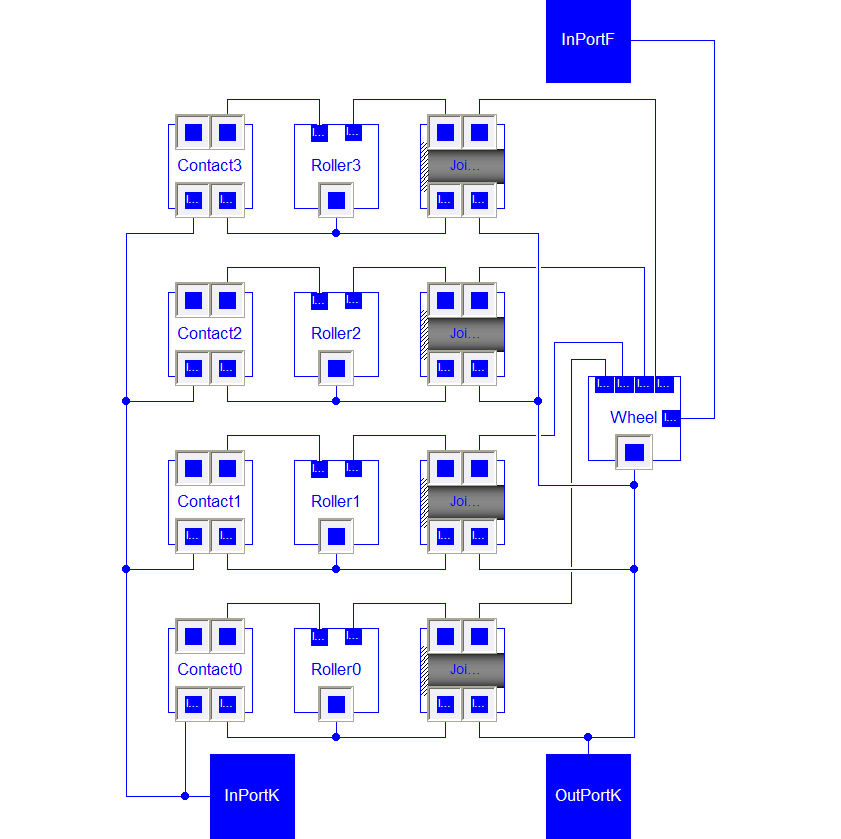
\includegraphics[bb= 0 0 19.50cm 20cm,scale=0.63]{OmniWheelModel.png}
%\centerline{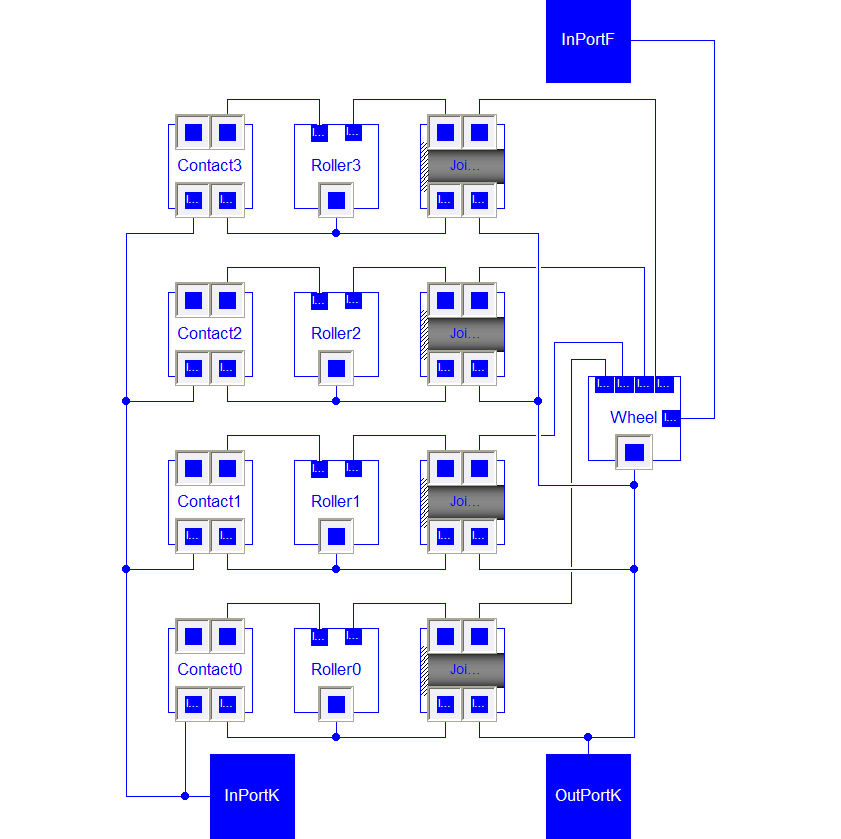
\includegraphics[bb= 0 0 19.50cm 20cm,scale=0.62]{OmniWheelModel.png}}
\caption{The omni wheel dynamics visual model.}
\end{center}
\label{VisualModel}
\end{figure}

\section{Implicit contact tracking algorithm}

We will assume in the further course that the wheel plane keeps its vertical 
orientation permanently. We have to introduce auxiliary orthonormal bases:
$b_1=\{ {\bf i}_1,{\bf j}_1,{\bf k}_1\} $ and 
$b_2=\{ {\bf i}_2,{\bf j}_2,{\bf k}_2\} $. Intermediate base $b_2$ 
characterises partially position and orientation of the roller, while the base
$b_1$ relates to the omni wheel.

The base $b_2$ coordinate system has its origin $O_B$ at the roller central
point. The unit vector ${\bf i}_2$ is directed along the roller axis of 
rotation, see Fig.~\ref{figure2}, fragment (a). The unit vector ${\bf j}_2$ is 
directed orthogonally to ${\bf i}_2$ and lies simultaneously in the vertical 
plane. Provided unit vectors ${\bf i}_2$, ${\bf j}_2$ are known the third unit 
vector ${\bf k}_2$ of the base $b_2$ is defined in a natural way as
\begin{equation}
{\bf k}_2={\bf i}_2\times {\bf j}_2.\label{k_2}
\end{equation}

\begin{figure}[htb]
\begin{center}
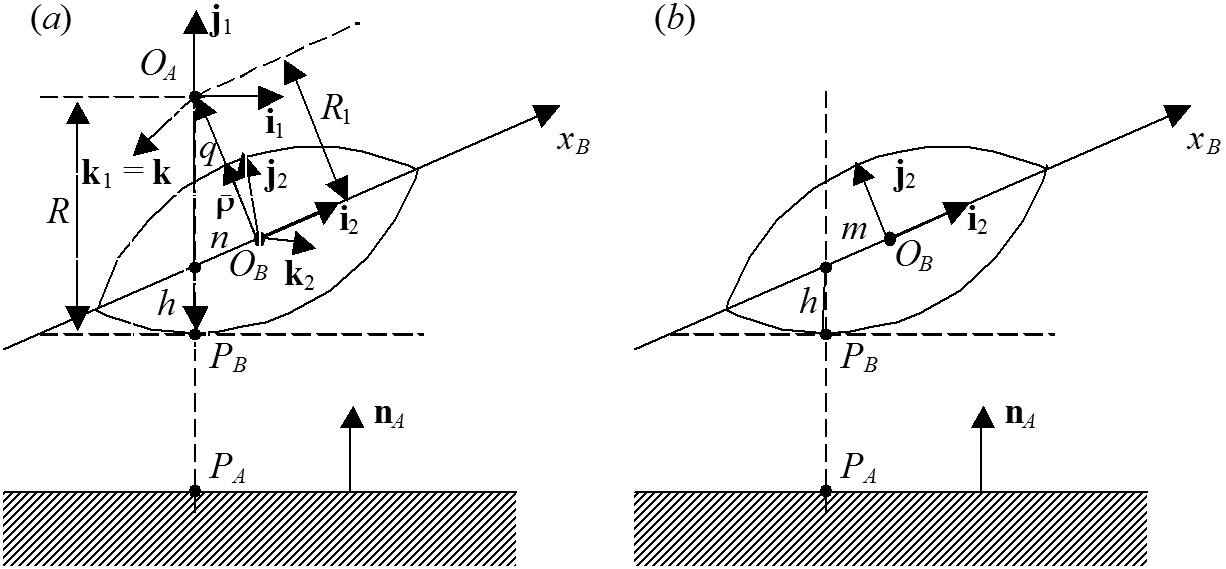
\includegraphics[bb= 0 0 19.50cm 10cm,scale=0.75]{ContactScheme.png}
\caption{Contact tracking scheme: (a) lateral view of the omni wheel with a 
roller has been rotated about line $O_AO_B$ by the angle $\psi $, (b) lateral 
view of the individual roller.}
\end{center}
\label{figure2}
\end{figure}

Remind here that all unit vectors are computed w.~r.~t. given fixed (absolute)
coordinate system. We assume that positions and orientations are known for all 
bodies belonging to the multibody system for any instant $t\in [t_0,t_1]$ of 
simulation process. Therefore, we have
\begin{equation}
{\bf i}_2=T_B\cdot (1,0,0)^T\label{i_2}
\end{equation}
where $T_B$ is the roller current orientation matrix.

Origin of the base $b_1$ coordinate system is located at the point $O_A$ ($=O$
in Fig.~\ref{figure1}) of the wheel center. The unit vector ${\bf i}_1$ 
is oriented horizontally and belongs to the wheel plane. The unit vector 
${\bf k}_1$ is orthogonal to the wheel plane and is identical to one of the 
wheel connected base vectors. We assume that using a controller the vector 
${\bf k}_1$ permanently maintains its horizontal state. Supposing vector 
${\bf k}_1(t)$ known we also have ${\bf j}_1(t)=(0,1,0)^T$ and 
${\bf i}_1(t)={\bf j}_1(t)\times {\bf k}_1(t)$.

Consider now relations providing base $b_2$ construction. Unit vector 
${\bf i}_2$ has been built above in~Eq.~(\ref{i_2}). During roller and the 
floor contact the vector ${\bf i}_2(t)$ can not become vertical. Moreover, if 
the roller distortion takes place, its angle of rotation $\psi >0$ about axis 
$O_AO_B$ is fixed non-zero, then the condition ${\bf i}_2\ne (0,1,0)^T$ is 
fulfilled permanently. So we can assume that the condition
\begin{equation}
{\bf c}={\bf i}_2\times (0,1,0)^T\ne {\bf 0}\label{c}
\end{equation}
is also fulfilled.

Thus using~Eq.~(\ref{c}) we can define ${\bf k}_2={\bf c}/|{\bf c}|$. And after 
this we can set ${\bf j}_2={\bf k}_2\times {\bf i}_2$. Geometrical constraints, 
conditions of orthogonality to be exact, play important role in the omni wheel 
kinematics
\begin{equation}
\bm\rho\cdot {\bf i}_2=0,\quad\bm\rho\cdot {\bf k}_1=0.\label{orth}
\end{equation}
where $\bm\rho =\left( {\bf r}_{O_A}-{\bf r}_{O_B}\right) /
\left| {\bf r}_{O_A}-{\bf r}_{O_B}\right|$. These equations actually are to 
compute the unit vector $\bm\rho $. Equations~(\ref{orth}) have their 
differential version
\begin{equation}
\Frac{d}{dt}\bm\rho\cdot {\bf i}_2+\bm\rho\cdot\Frac{d}{dt}{\bf i}_2=0,\quad
\Frac{d}{dt}\bm\rho\cdot {\bf k}_1+\bm\rho\cdot\Frac{d}{dt}{\bf k}_1=0.
\end{equation}

The value $c_{\beta }=\cos\beta ={\bf i}_2\cdot (0,1,0)^T$ of cosine for the 
angle $\beta $ of the roller axis inclination to vertical $(0,1,0)^T$ plays 
also an important role in the contact tracking algorithm. If current value of
the variable $c_{\beta }$ is less than some limiting parameter 
$c_{\beta\max }$, and simultaneously if an altitude of the point $O_B$ defining
position of the roller center is less than value $R$ of the wheel radius then
the contact takes place. Otherwise no contact occurs.

Note here that in order to arrange the unilateral constraint in the multibody
system dynamics model the developer usually has to implement construct similar 
to hybrid automata. In our omni wheel model, on the contrary, this is not the 
case. It turned out sufficient to implement ``simple'' ``{\tt if}''-construct 
to switch states ``contact'' and ``no contact'' for each individual roller, and 
simultaneously to advance forward ``contact'' state from the roller-in-contact 
to its neighbour. The whole picture looks like from time to time neighbouring 
rollers mutually exchange their states. One can find details of the unilateral 
constraint implementation in~(Kosenko, 2015). Merely note that 
``{\tt if}''-alternatives are the following: (a) ``contact'' state corresponds 
to zero-valued relative normal acceleration of two contacting surfaces at the 
point of contact, (b) ``no contact'' branch corresponds to the zero-valued 
reaction mutual for both bodies at contact. All this is according to the 
so-called Signorini rule. ``{\tt if}''-condition depends on the roller 
orientation variables.

A contact tracking algorithm plays an essential role in all these computations.
Generally, its implementation reduces to computation of the contact point/patch
whitch enables computing forces at contact. Usually, one considers contact of 
two surfaces participating in rigid/elastic interaction of two massive bodies. 
As a rule, such algotithms are pretty expensive and noticeably slow while the 
whole simulation process. Fortunately, in case of omni wheels we found here the 
simplest way to make this computation as fast as possible using ``elementary'' 
geometric considerations.

We can also easily see from the Fig.~\ref{figure2} that the point $P_B$ of 
contact between roller and floor is obtained using formula
\begin{equation}
{\bf r}_{P_B}={\bf r}_{O_B}+R_1\bm\rho -R{\bf j}_1+\mu {\bf k}_1,\label{R_1}
\end{equation}
where the scalar $\mu $ is to be computed. The value $R_1$ in~Eq.~(\ref{R_1}) 
is the distance between points $O_A$ and $O_B$. The scalar $\mu $ can be 
computed if we multiply the last equation by ${\bf k}_2$ using dot-product. 
Thus we have
\begin{equation}
\mu =\left[R{\bf j}_1\cdot{\bf k}_2-R_1{\bm\rho }\cdot {\bf k}_2\right] /
{\bf k}_1\cdot{\bf k}_2
\label{mu}
\end{equation}
since the vector ${\bf r}_{P_B}-{\bf r}_{O_B}$ lies in vertical section of
axisymmetrical surface of the roller, and the vector ${\bf k}_2$ 
in~Eq.~(\ref{mu}) by construction is orthogonal to this section. As a result 
the position ${\bf r}_{P_B}$ of the contact point $P_B$ is uniquely computed.

\section{Explicit contact tracking algorithm}

Yet another way to obtain current position ${\bf r}_{P_B}$ of the contact point
$P_B$, or more accurately: the roller point closest to the floor, is an 
application of the following chain of equations. This chain is simply
understood from geometrical scheme shown in Fig.~\ref{figure2}, (a) and (b),
such that
\begin{equation}
{\bf r}_{P_B}={\bf r}_{O_B}-m{\bf i}_2-h{\bf j}_1,
\label{expl}
\end{equation}
where $m=R_1\sin q/\cos q/\cos\psi $, $h=R-R_1/\cos q$, $q$ is the current 
value for angle of deviation of the vector $\bm\rho$ from direction of the 
vector ${\bf j}_1$. Really it is an angle of the wheel rotation being counted
from the local vertical. So using~Eq.~(\ref{expl}) we have formulae
\begin{equation}
\cos q=\bm\rho\cdot{\bf n}_A,\quad\sin q=
\left({\bf n}_A\times\bm\rho\right)\cdot {\bf k}_1.
\label{q}
\end{equation}

Resulting from~Eqs.~(\ref{expl}), (\ref{q}) further we proceed with 
explanations of some details in Fig.~\ref{figure2}. Fragment (a) corresponds to 
the lateral projection of the wheel and likewise the distorted roller 
projection. This latter object is shown here in a general position. 
Furthermore, $P_B$ is the current contact point between the roller and the 
horizontal floor, $n$ is a projection of the roller axial line segment onto the 
wheel plane. We can see easily that this projection is computed by the formula 
$n=m\cos\psi $ because the roller axis is turned about $O_AO_B$ by the angle 
$\psi $, see fragment (b) for the roller axial vertical lateral section. Thus, 
we have to pass two straight line segments from the roller center $O_B$ 
to reach the point $P_B$: (a)~the segment of the roller axis of length $m$; 
(b)~the segment down the vertical of length $h$. As we already mentioned above
all variables needed are computed through known variables using explicit 
formulae.

In case of $\psi >0$, distortion exists, for both implicit and explicit 
algorithms not all the length of the roller surface generatrix is necessarily
in contact. So really we have to cut tips of rollers to provide regular
simulation process. We can obtain length of the tip to be cut for instance 
empirically or compute it explicitly. Indeed, one can easily see from 
Fig.~\ref{figure2} that the real roller length should be computed by the
formula $L=2R\sin\alpha /\cos\psi $.

``Ideal'' switching of contact takes place in this case: exactly at the instant 
of contact loss for current roller a contact immediately arises for the 
``next'' roller in direction of the wheel rolling.

\section{Description of the roller surface geometry}

The roller surface is defined as a surface of rotation. An arc of the circle
having radius $R$ becomes a generatrix for this surface in case of the roller
axis belongs to the omni-wheel plane. In case of the roller axis inclined 
position the roller surface generatrix shape is more complicated.

Assume the coordinate system $OXYZ$ being interconnected with the wheel 
rigidly, see~Fig.~\ref{Fig3}. Axis $OZ$ is assumed to be directed along the 
wheel axis of rotation. We will suppose that the wheel rolls on the horizontal 
surface and its plane $OXY$ keeps its vertical orientation permanently. 
Consider roller which axis midpoint $C$ lies on the axis $OY$ by the distance 
$R-r$ from $O$. The roller axis of rotation $Cx$ intersects $OY$ under the 
right angle and is inclined to the plane $OXY$ by the angle $\psi $. Denote 
here as $A$ and $B$ the points of the axis $Cx$ intersection with the cylinder 
$H={X^2+Y^2=R^2}$. Also assume that $AB=2l$. Projection of the segment $AB$ 
onto the plane $OXY$ has a length $2l'=2l\cos\psi $. And this segment component 
orthogonal to the plane $OXY$ has a length $2l\sin\psi $. Lateral view, along 
the axis $OZ$, of the segment $AB$ and cylinder $H$ is shown 
in~Fig.~\ref{Fig3}, detail a). Top view from above is shown in~Fig.~\ref{Fig3}, 
detail c). Vertical section of the roller along the segment $AB$ is shown 
in~Fig.~\ref{Fig3}, detail b).

\begin{figure}[h]
%\begin{center}
\centerline{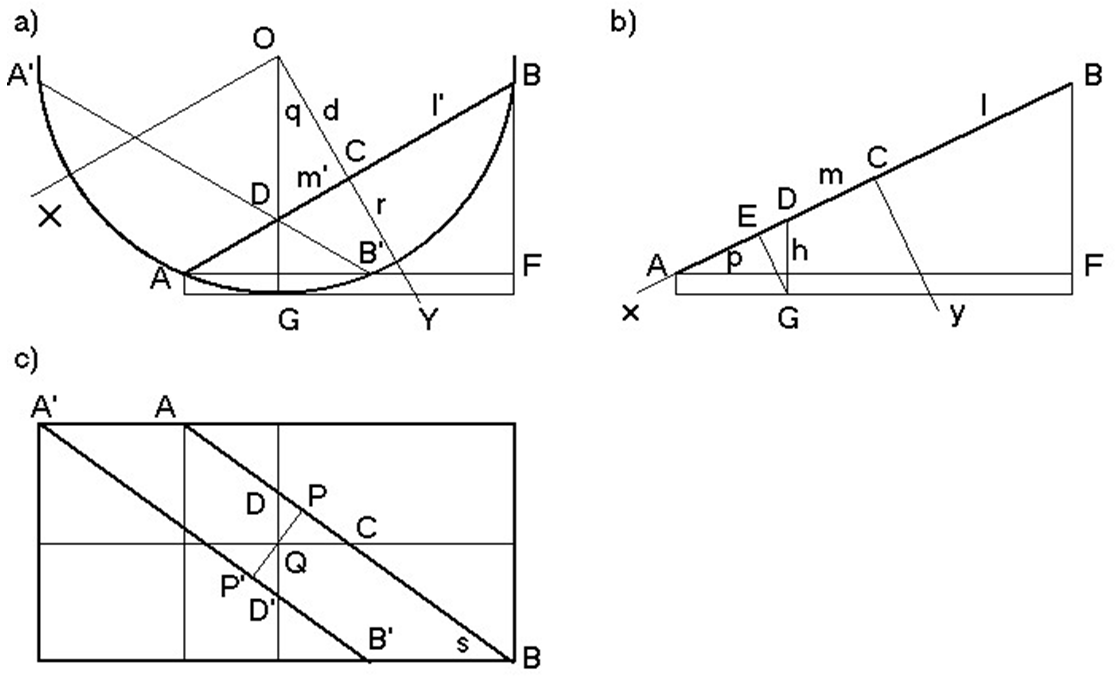
\includegraphics[bb = 0 0 19.50cm 12cm,scale=0.7]{RollerGeometry.png}}
\caption{The roller contact surface geometry.}
%\end{center}
\label{Fig3}
\end{figure}

Here, in detail a), $q$ is the angle of the wheel rotation about the axis $OZ$
counting from the roller horizontal position, $D$ is the point the segment $AB$
intersection with the vertical plane including $OZ$. In Fig.~\ref{Fig3}, detail 
a), vertical coordinates of points are equal to the vertical coordinates of the 
corresponding points in detail b). Simultaneously, horizontal dimensions are 
compressed with the coefficient such that relations $l'=l\cos\psi $ and 
$m'=m\cos\psi $ fulfil. From the angled triangle $OCD$ projection a) and from 
relation between the triangle $ABF$ projections a) and b) one has
\begin{equation}
m'=(R-r)\tan q,\quad m=(R-r)\tan q/\cos\psi ,\quad h=R-(R-r)/\cos q,\quad
\sin p=\sin q\cos\psi .
\label{aux}
\end{equation}

Using~Eq.~(\ref{aux}) one can define the roller surface generatrix as a locus 
$G$ for the angle $q$ being varied in the coordinate system $Cxy$ of the 
vertical plane from the Fig.~\ref{Fig3}, detail b), in the following way 
$x=CE=m+h\sin p$, $y=EG=h\cos p$, or
$$
x(q)=R\cos\psi +(R-r)\left(\Frac{1}{\cos\psi }-\cos\psi\right)\tan q,\quad
y(q)=\left(R-\Frac{R-r}{\cos q}\right)\sqrt{1-\cos ^2\psi\sin ^2q}.
$$

\section{The wheel model classes hierarchy}

Model of the omni wheel testbench virtual prototype is a container class 
including the following objects instantiated: (a)~disk of the wheel; 
(b)~objects of rollers mounted along the wheel rim; (c)~objects of joints
connecting rollers and the wheel disk; (d)~objects of contacts connecting 
objects of rollers and the object of the horizontal floor surface; (e) model of
base body as a horizontal floor.

Let us analyse in more details a structure of contact model. This model has
many similarities with contact models including contact tracking algorithms of
general case previously considered in~(Kosenko, 2006). Nevertheless important 
differencies exist. One of them mentioned above with regard to organization of 
the contact class using simple and efficient construct of contact 
tracking~(Kosenko, 2015). Note that in case of $\psi >0$ the point of contact 
creates a curve with discontinuities at instances of rollers changes. However, 
this circumstance does not prevent the process of regular simulation.

\begin{figure}[h]
\centerline{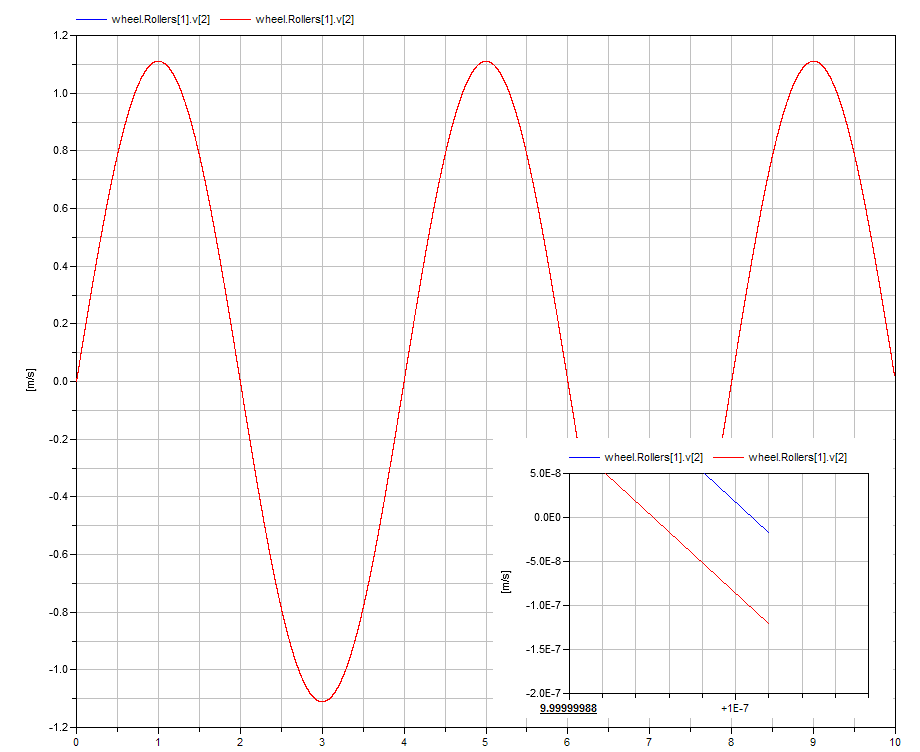
\includegraphics[bb= 0 0 19.50cm 16cm,scale=0.75]{VelocityDiverg.png}}
\caption{Comparison of dynamics for the roller No. 1 central point, its 
velocity $y$-coordinate, for cases of: explicit (blue curve) and implicit (red 
curve) algorithm of contact tracking.}
\label{figure5}
\end{figure}

\begin{figure}[h]
\centerline{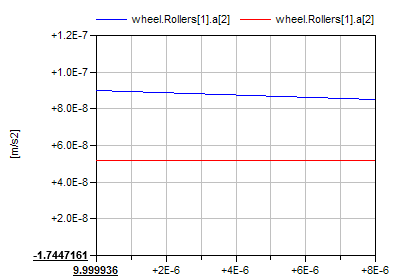
\includegraphics[bb= 0 0 19.50cm 14cm,scale=0.45]{AccDiv.png}}
\caption{Divergence for $y$-components of acceleration.}
\label{figure6}
\end{figure}

\begin{figure}[h]
\centerline{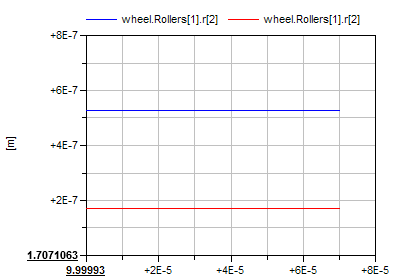
\includegraphics[bb= 0 0 19.50cm 14cm,scale=0.45]{PosDiv.png}}
\caption{Divergence for $y$-components of position.}
\label{figure7}
\end{figure}

Finally, we apply rigid point contact model as part of the simplest omni wheel
model. For this we use the base class for constraint/contact models having only
equations of Newton's third law as a behavioral section~(Kosenko, 2007). We use 
class of the contact tracking model on the second stage of inheritance. Cases 
of this class organization have been analysed above. Coordinates of nearest 
points $P_A$ and $P_B$ at contact for each pair (floor, roller) are computed as 
a result for this class functionality.

Class for computing all kinematical characteristics at contact needed ``works''
in case of contact existence on the next stage of inheritance. On the third
stage class for computing the reactions at contact is ``turned on''. Reactions 
are the following: (a) normal reaction; (b) tangent force of friction; (c) 
torque of reactions (zero in the current consideration though it is not 
difficult to compute torque for several contact models). One can reconstruct 
the total sequence of inheritance for classes menioned above in a following 
way: {\tt Constraint} (Contact Base Class) is the base class for: {\tt Contact 
Tracking Model} which is the base class for: {\tt Class of Kinematics} which is 
the base class for: {\tt Class of Reactions} which is the last in the sequence 
of derived classes.

For each roller of the omni wheel model when contacting the friction model 
being used is �turned on�. In our model being developed the ``simple'' law of 
the Amontons -- Coulomb dry friction is applied. Actually we use known 
piecewise approximation (Kosenko, 2006) to exact dry friction instead. This 
approximation has high accuracy over long time intervals (Novozhilov, 1997).

All constructs enumerated above were implemented using Modelica language of
object-oriented modeling~(Fritzson, 2004) in frame of the visual compiler with
simulation environment Dymola~(Dymola, 2004) with use of so-called 
physically oriented approach~(Cellier~et~al, 1996), (Kosenko, 2007).

To verify an approach for building up the models under analysis we compare the
omni wheel dynamics in cases of implicit and explicit algorithms. The wheel 
performs free motion (combining rotation and sliding) with the only 
restriction: keep vertical alignment of the wheel disk.

Roller No.~1 central point, its mass center, altitude was analyzed and 
verified. More accurately we examine $y$-coordinate of the point velocity. Both 
models turned out almost identical: in the worst case we have a divergence: in
accelerations of order $10^{-8}$, in velocities of order $10^{-7}$, in position
of order $10^{-6}$ over the time span being equal to 10 units of time. Results 
of simulation for velocities are shown in Fig.~\ref{figure5}. Other 
divergencies for the roller No.~1 central point acceleration and position at 
time = 10units are shown in Fig.~\ref{figure6} and~\ref{figure7} respectively. 
As expected the model with explicit contact tracking algorithm is faster 
approximately in $1.5$ times.

\section{Conclusions}

The following effects were found as a results of new contact tracking 
algorithms applying to the omni wheel multibody system:
\begin{enumerate} 

\item
Two contact tracking algorithms were proposed: implicit and explicit. As
expected the second algorithm turned out to be faster almost in $1.5$ times. 
Both algorithms are simple (and efficient) even in simpler case of rollers 
without any distortion.

\item
In case of distorted rollers contact curve becomes discontinuous at instants
of rollers change. But simulation process maintains its regularity.

\item
Both implicit and explicit contact tracking algorithms generate identical 
dynamics.

\item
Process of the contact model design using a technology of the so-called 
``vertical foliation'' outlined above has an evident motivation and allows a 
simple generalization both for the normal force computation and for the tangent 
friction force model.

\end{enumerate} 

\section{Acknowledgement}

The investigation was performed in MAI under financial support provided by RSF, 
project 14-21-00068.

\begin{thebibliography}{99}

\bibitem{Cellier, 1996}
Cellier, F. E., Elmqvist, H., and Otter, M., Modeling from Physical Principles, 
In: Levine W. S. (Ed.), The Control Handbook, CRC Press (1996), pp.99--107.

\bibitem{Dymola, 2009}
Dymola. Dynamic Modeling Laboratory. User Manual. Volumes 1 and 2. Dymola 7.3, 
Dynasim AB, Research Park Ideon, Lund, (2009).

\bibitem{Fritzson, 2004}
Fritzson, P., Principles of Object-Oriented Modeling and Simulation with 
Modelica 2.1, IEEE Press, (2004).

\bibitem{Ilon, 1975}
Ilon, B. E., Wheels for a Course Stable Selfpropelling Vehicle Movable in Any
Desired Direction on the Ground or Some Other Base. Technical report, US 
Patents and Trademarks office, Patent 3,876,255, (1975).

\bibitem{Kalman, 2013}
K\'alm\'an, V., Controlled Braking for Omnidirectional Wheels, International 
Journal of Control Science and Engineering, Vol.3, No.2 (2013), pp.48--57.

\bibitem{Komori, 2016}
Komori, M., Matsuda, K., Terakawa, T., Takeoka, F., Nishihara, H., and Ohashi, 
H., Active Omni Wheel Capable of Active Motion in Arbitrary Direction and 
Omnidirectional Vehicle, Journal of Advanced Mechanical Design, Systems, and 
Manufacturing,  Vol.10, No.6 (2016), pp.1--20.

\bibitem{Kosenko, 2006}
Kosenko, I. I., Implementation of Unilateral Constraint Model for Multibody 
Systems Dynamics on Modelica Language, Proceedings of ACMD2006, The Third Asian 
Conference on Multibody Dynamics 2006, Institute of Industrial Science, The 
University of Tokyo, Tokyo, Japan, August 1--4 (2006), 8~pp.

\bibitem{Kosenko, 2007}
Kosenko, I. I., Physically Oriented Approach to Construct Multibody System 
Dynamics Models Using Modelica Language, Proceedings of Multibody 2007, 
Multibody Dynamics 2007. An ECCOMAS Thematic Conference, Politecnico di Milano, 
Milano, Italy, June 25--28 (2007), 20~pp.

\bibitem{Kosenko, 2015}
Kosenko, I. and Gerasimov, K., Object-Oriented Approach to the Construction of 
an Omni Vehicle Dynamical Model, Journal of Mechanical Science and Technology, 
Vol.29, Iss.7 (2015), pp.2593--2599.

\bibitem{Novozhilov, 1997}
Novozhilov, I. V., Fractional Analysis: Methods of Motion Decomposition,
Birkhauser, (1997).

\bibitem{Tobolar, 2009}
Tobol\'ar, J., Herrmann, F. and B\"unte, T., Object-Oriented Modelling and 
Control of Vehicles with Omni-Directional Wheels, Computational Mechanics 2009, 
November 2009.

\bibitem{Zobova, 2009}
Zobova, A. A., Tatarinov, Ya. V., The Dynamics of an Omni-Mobile Vehicle, 
Journal of Applied Mathematics and Mechanics, Vol.73, Iss.1 (2009), pp.8--15.

\end{thebibliography}

\end{document}
